\begin{center} 
	\textbf{\myappendix{User's Manual}}
\end{center}

\noindent
\textbf{Accesing the System}
\begin{enumerate}
	\setstretch{1}
	\item[1.] Install Xampp version 5 or latest
	\item[2.] Run Apache and MySQL
	\item[3.] Go to localhost/new
\end{enumerate}

\noindent
\textbf{Loggin In \\}
\begin{center}
	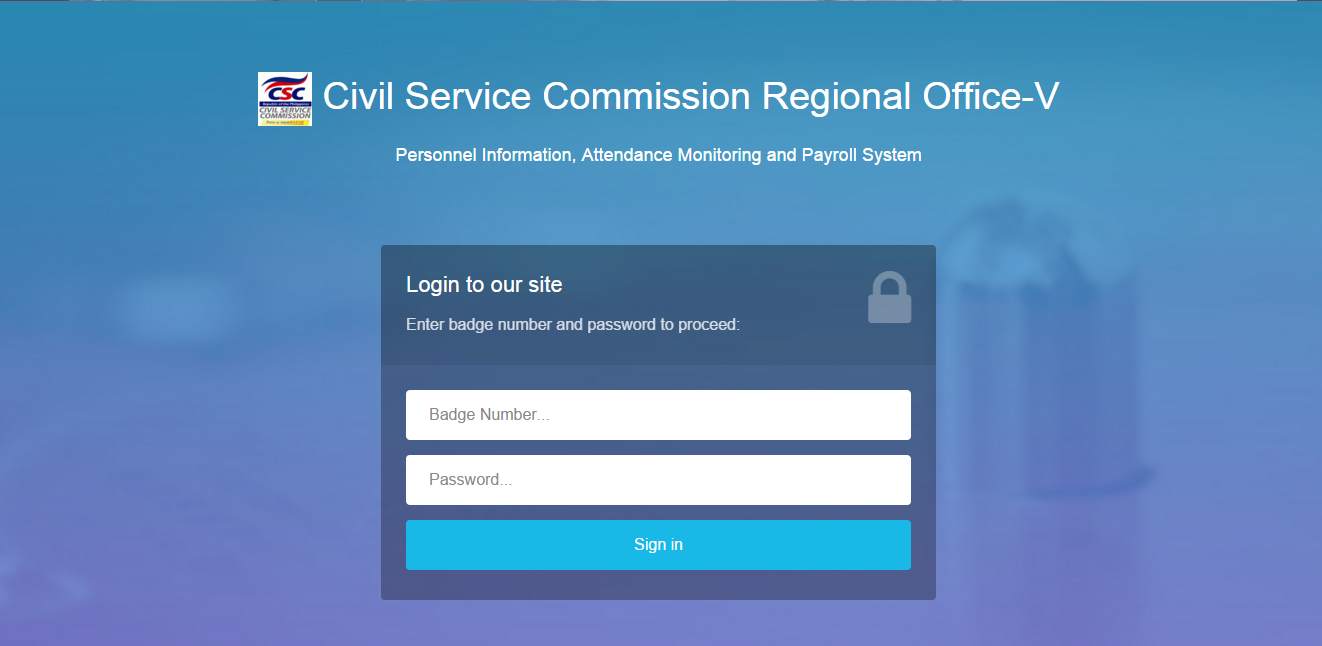
\includegraphics[width=15cm,height=6cm]{image/login.png}
\end{center}

Ask for your badge number from the Admin, the default password is "password".

\newpage
\noindent
\textbf{ Profile \\}
\begin{center}
	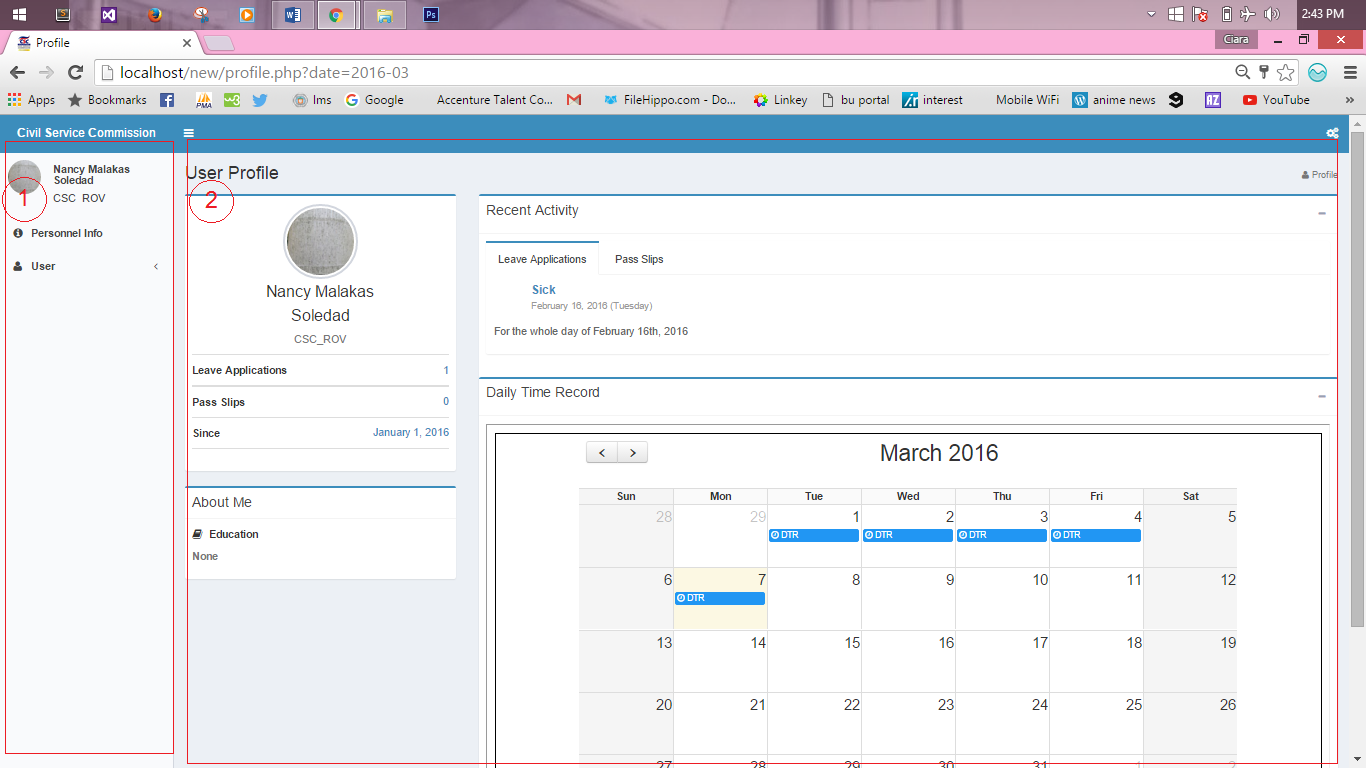
\includegraphics[width=15cm,height=7cm]{image/profile_user.png}
\end{center}

Shown in your profile are 2 panes. The \textbf{left pane} contains all the features or functions you are allowed to do. The \textbf{main pane} contains your personal details, list of all your filed applications and a calendar.

\noindent
\textbf{ 1. Left Pane \\}

\noindent \textbf{User (This option is available to all users) }
\begin{itemize}
	\item Manage and View Payslip – You can view this month’s Payslip or select which month’s Payslip you want to view. \\
	\begin{center}
		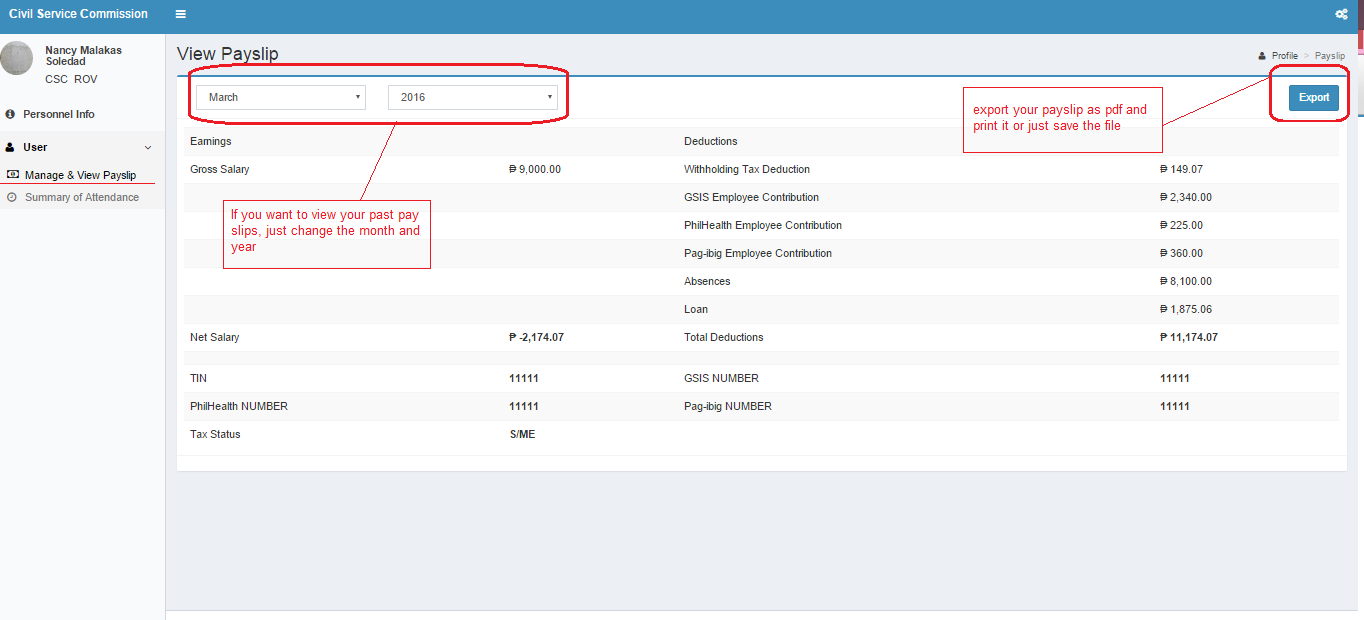
\includegraphics[width=15cm,height=7cm]{image/viewPaySlip.png}
	\end{center}
	
	
	\item Summary of Attendance - you can view the summary of your attendance, the total late, undertime and absences for the month. \\
	\begin{center}
		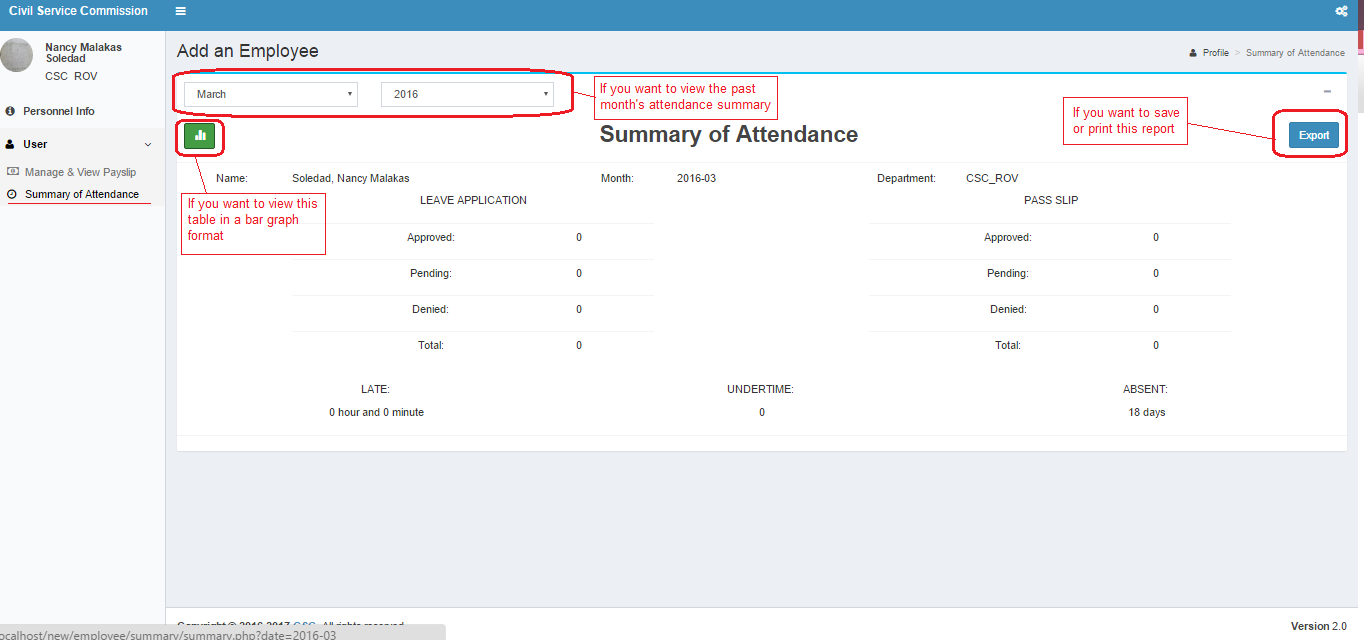
\includegraphics[width=15cm,height=7cm]{image/summaryOfAttendance.png}
	\end{center}
	
\end{itemize}
\newpage
\noindent
\textbf{Personnel Information (Only available for Personnel Information Admins and Superadmin) \\}
\begin{center}
	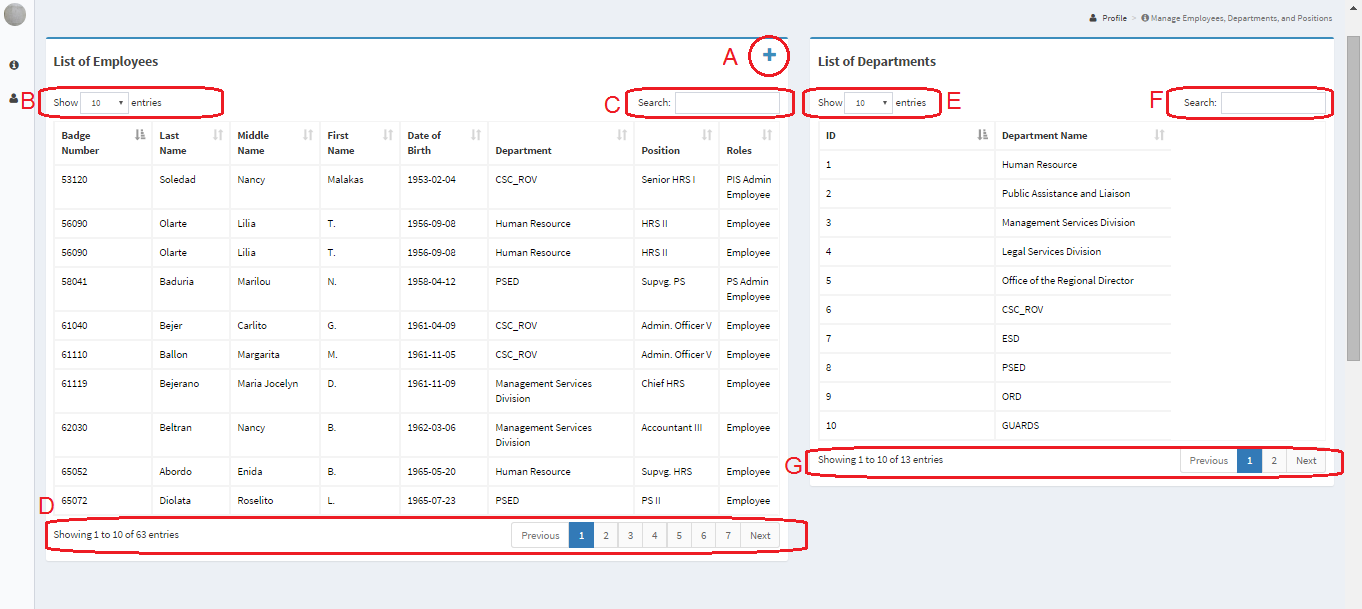
\includegraphics[width=15cm,height=7cm]{image/PISadmin1.png}
\end{center}

\begin{itemize}
	\item List of Employees
	\begin{enumerate}
		\item[A.] Add an Employee - click the “+” button on the upper right corner. A window will appear where you can enter basic information about the employee \\
		\begin{center}
			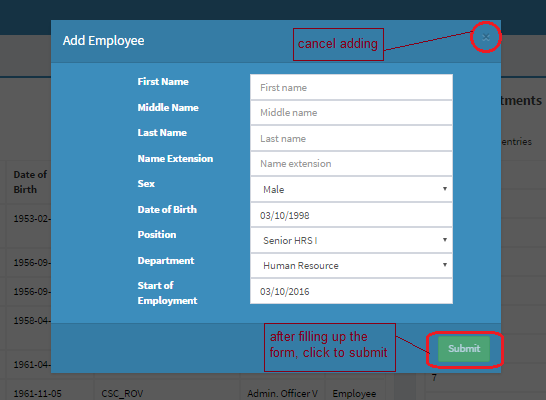
\includegraphics[width=8cm,height=8cm]{image/addemp_um.png}
		\end{center}
		
		\item[B.] Show - Click the arrow down button beside the number and choose how many entries you want to view.
		\item[C.] Search - On the textfield type the keyword. It will find the keyword in al the columns.
		\item[D.] Number of Entries and Pages - Shown is the number of entries shown and the total number of entries. The number of pages is also shown, click the page number to view the entries on that page.
	\end{enumerate}
	\item List of Departments
	\begin{enumerate}
		\item[E.]Show - Click the arrow down button beside the number and choose how many entries you want to view.
		\item[F.] Search - On the textfield type the keyword. It will find the keyword in al the columns.
		\item[G.] Number of Entries and Pages - Shown is the number of entries shown and the total number of entries. The number of pages is also shown, click the page number to view the entries on that page.
	\end{enumerate}
\end{itemize}
\begin{center}
	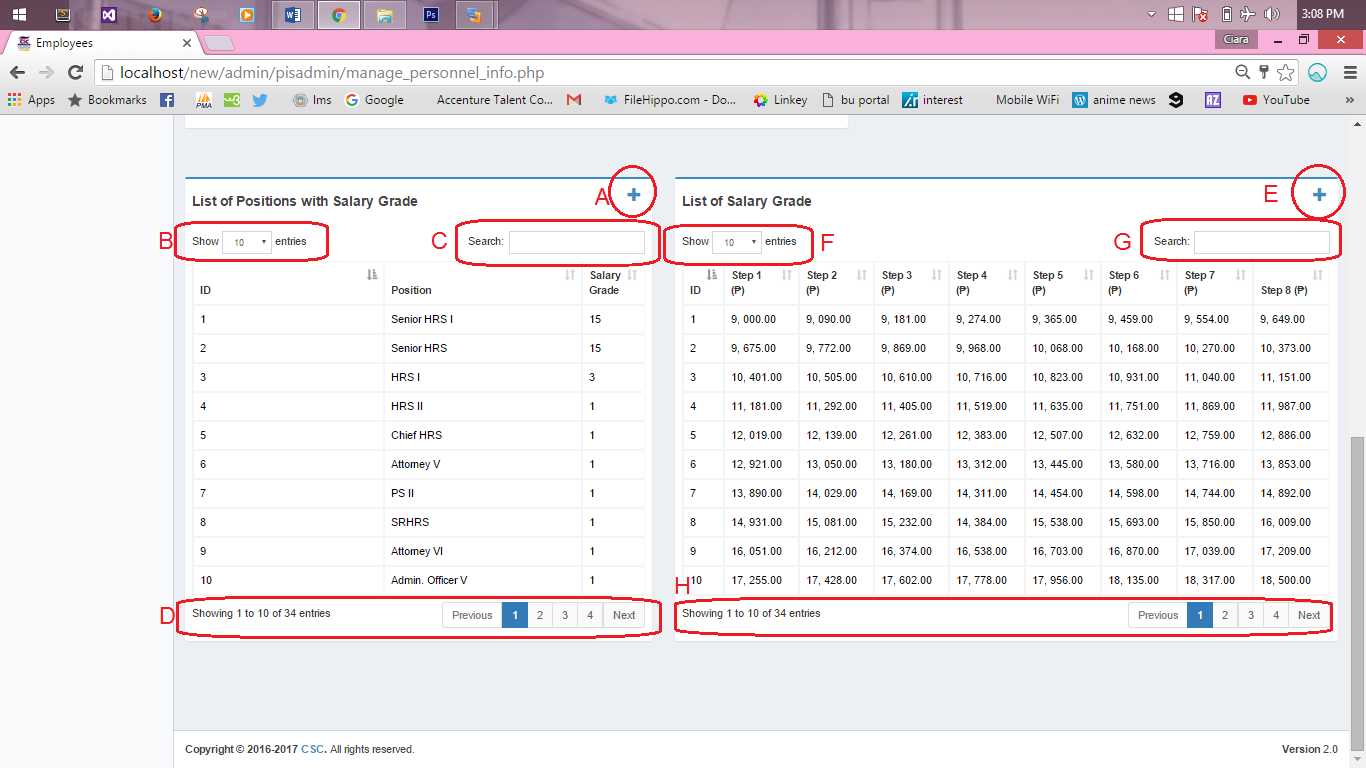
\includegraphics[width=15cm,height=7cm]{image/PISadmin2.png}
\end{center}
\begin{itemize}
	\item List of Positions with Salary Grade 
	\begin{enumerate}
		\item[A.] Add - click the “+” button on the upper right corner. A window will appear where you can enter the position name , the default salary grade is 1. you can edit it later.\\
		\begin{center}
			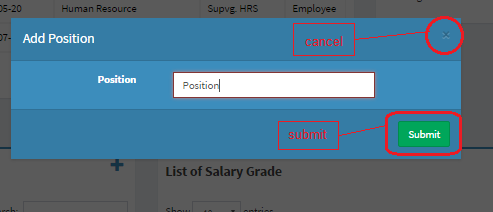
\includegraphics[width=8cm,height=4cm]{image/addpos_um.png}
		\end{center} 
		\item[B.] Show - Click the arrow down button beside the number and choose how many entries you want to view.
		\item[C.] Search - On the textfield type the keyword. It will find the keyword in al the columns.
		\item[D.] Number of Entries and Pages - Shown is the number of entries shown and the total number of entries. The number of pages is also shown, click the page number to view the entries on that page.
	\end{enumerate}
	\item List of Salary Grade
	\begin{enumerate}
		\item[E.] Add - click the “+” button on the upper right corner. A window will appear where you can enter the amount for the 8 steps\\
		\begin{center}
			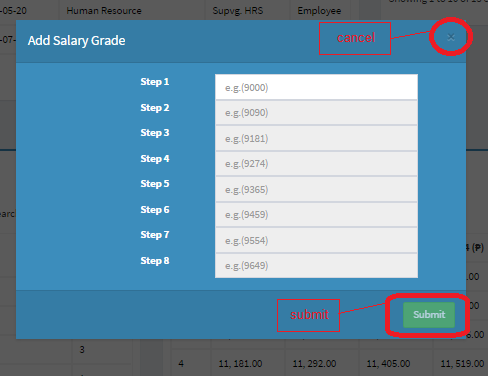
\includegraphics[width=8cm,height=7cm]{image/addsalarygrade_um.png}
		\end{center} 
		\item[F.] Show - Click the arrow down button beside the number and choose how many entries you want to view.
		\item[G.] Search - On the textfield type the keyword. It will find the keyword in al the columns.
		\item[H.] Number of Entries and Pages - Shown is the number of entries shown and the total number of entries. The number of pages is also shown, click the page number to view the entries on that page.
	\end{enumerate}
\end{itemize}
\newpage
\noindent
\textbf{Attendance Monitoring (Available to Attendance Monitoring System Admins and Superadmin only)\\ }
\begin{center}
	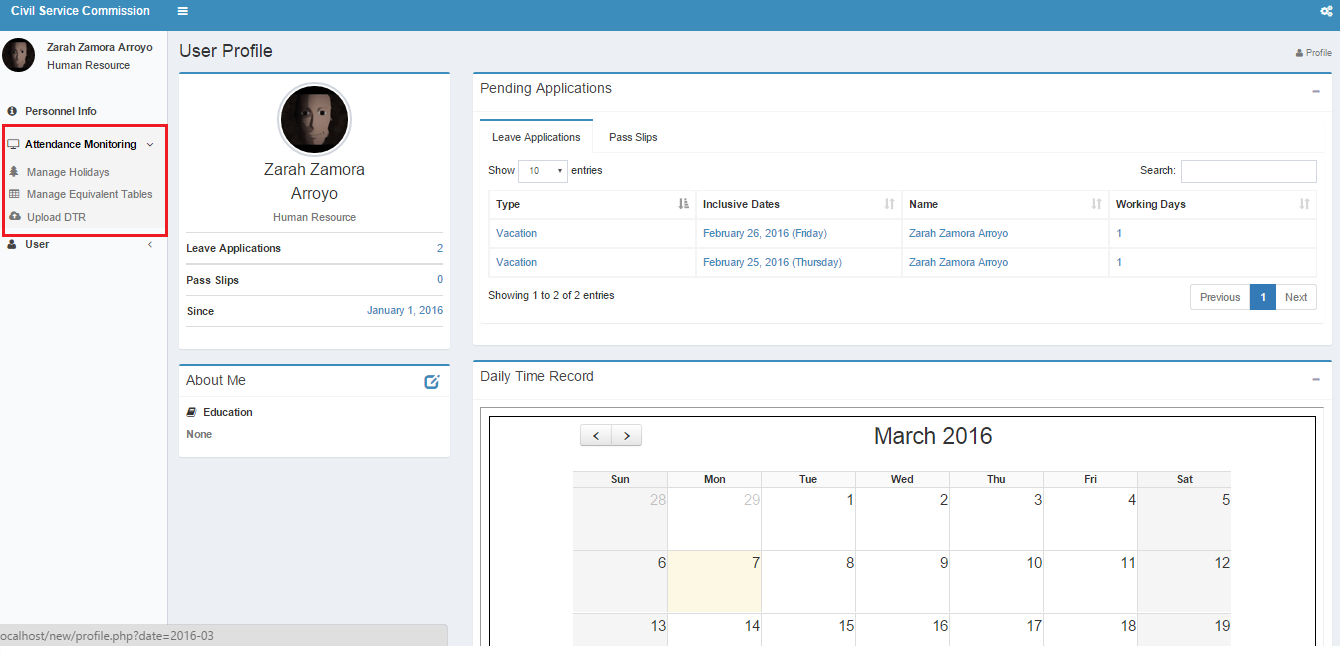
\includegraphics[width=14cm,height=7cm]{image/ams_um.png}
\end{center} 
\begin{enumerate}
	\item[A.] Manage Holidays -Add or Edit the holidays and Special Events. \\
	\begin{center}
		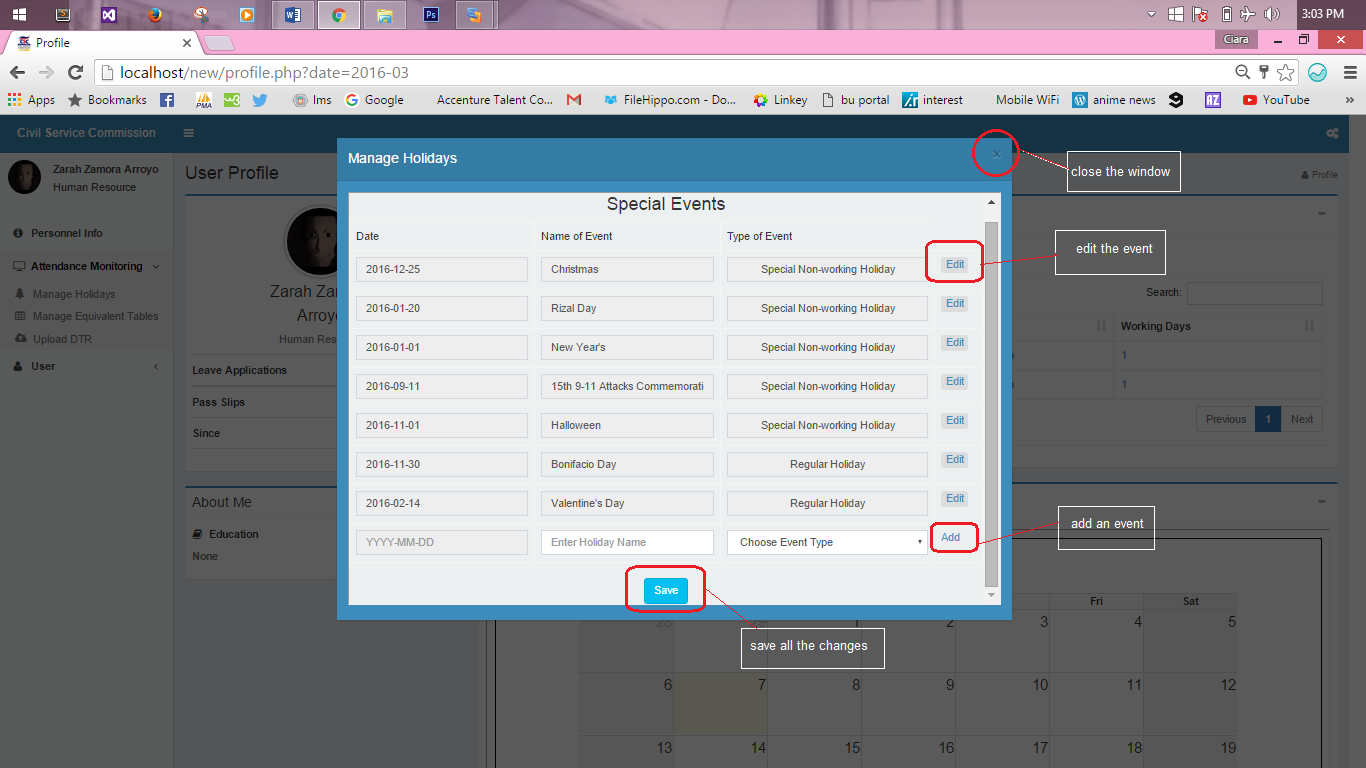
\includegraphics[width=14cm,height=7cm]{image/Holidays.png}
	\end{center}
	\item[B.] Manage Equivalent Tables – Edit the Equivalent table for Leave Credits. \\
	\begin{center}
		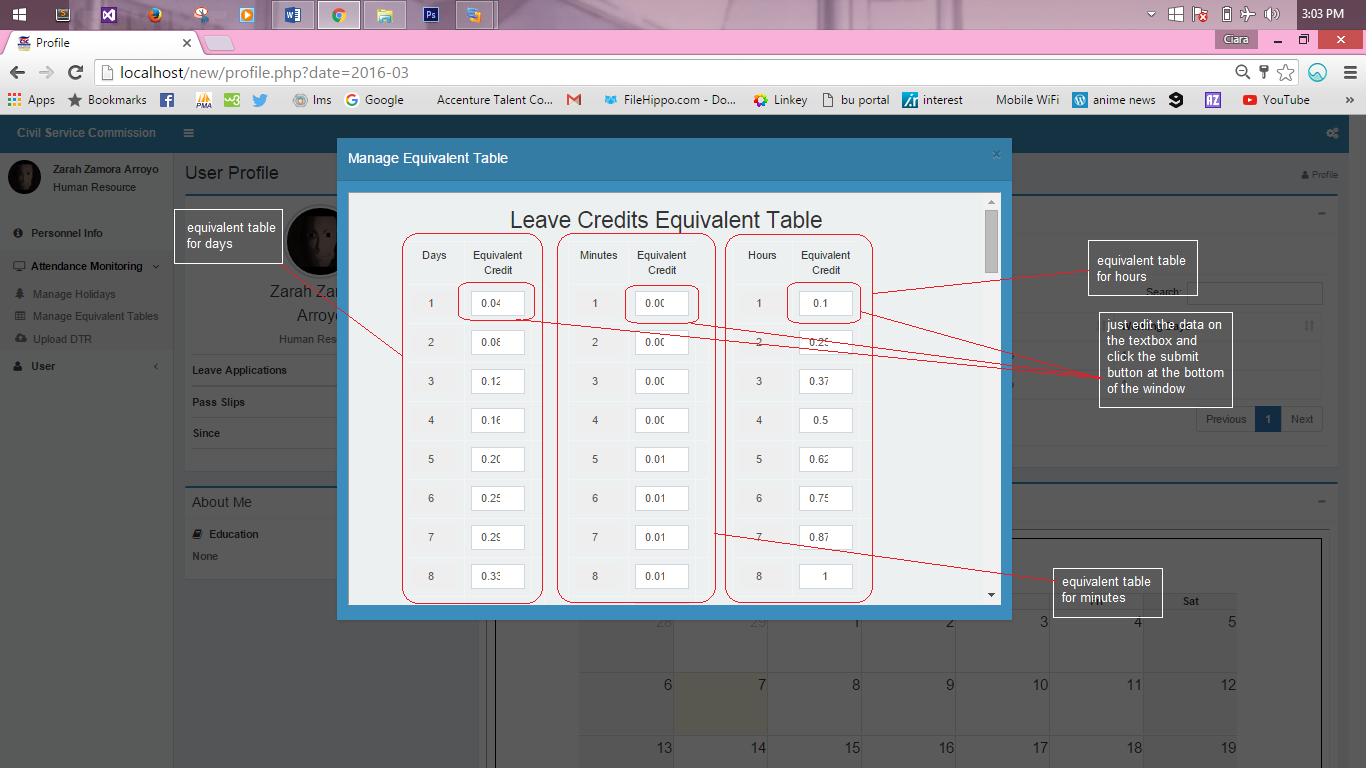
\includegraphics[width=14cm,height=7cm]{image/LCequi.png}
	\end{center}
	\item[C.] Upload DTR – this option is for uploading the CSV file from the Biometrics. \\
	\begin{center}
		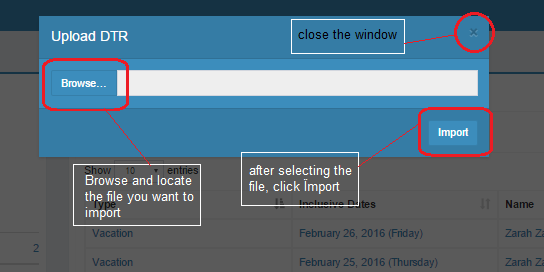
\includegraphics[width=8cm,height=4cm]{image/upload.png}
	\end{center}
\end{enumerate}
\newpage
\noindent
\textbf{Payroll (Available to Payroll System Admins and Superadmin only) \\}
\begin{center}
	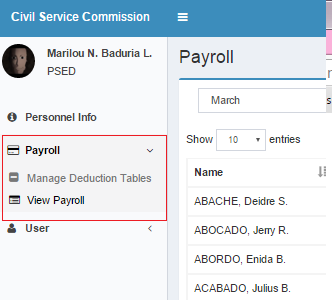
\includegraphics[width=7cm,height=7cm]{image/PS_um.png}
\end{center} 

\begin{enumerate}
	\item[A.] Manage Deduction Tables – Manage the deduction tables for PAG-IBIG, PhilHealth, Tax and GSIS.
	\begin{center}
		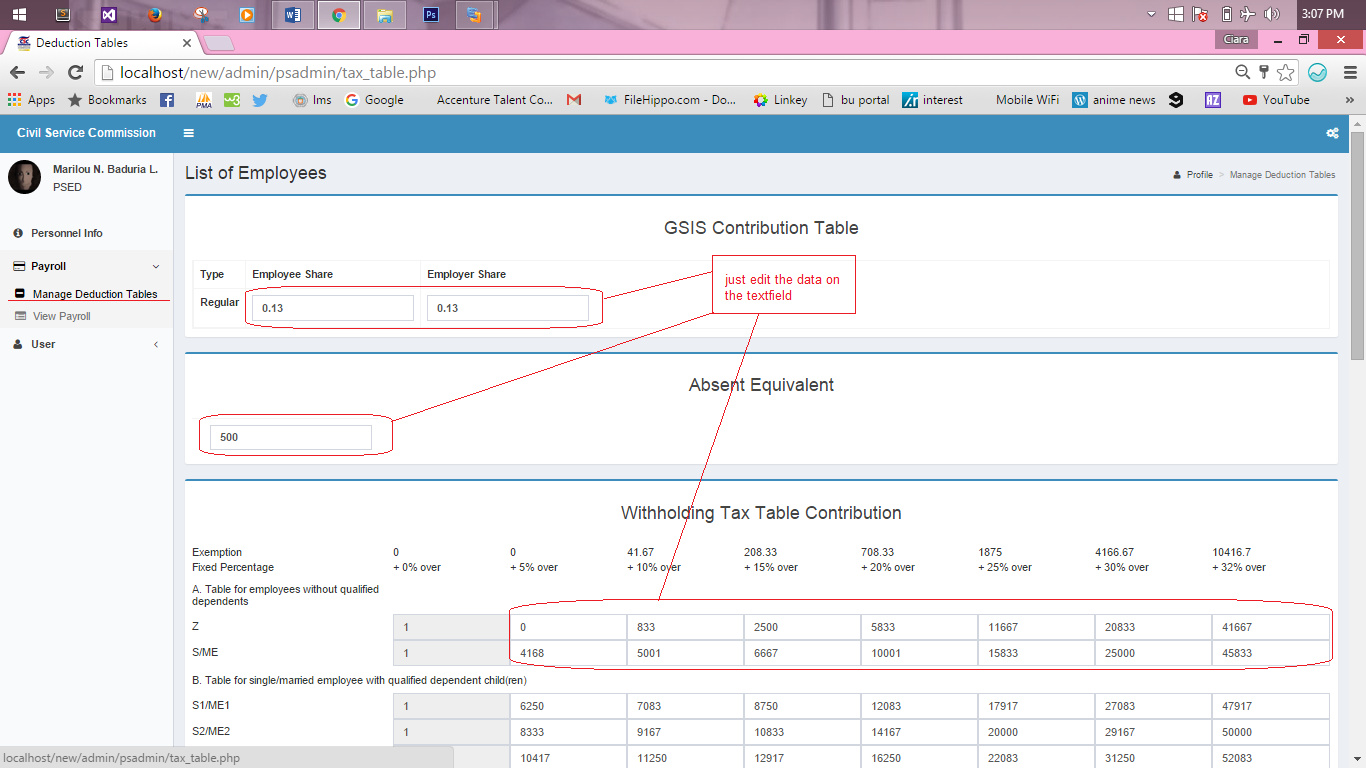
\includegraphics[width=14cm,height=7cm]{image/deducTables.png}
	\end{center} 
	\item[B.] View Payroll -  View the Payroll which contains a list of employees with their gross pay, deductions and net pay.
	\begin{center}
		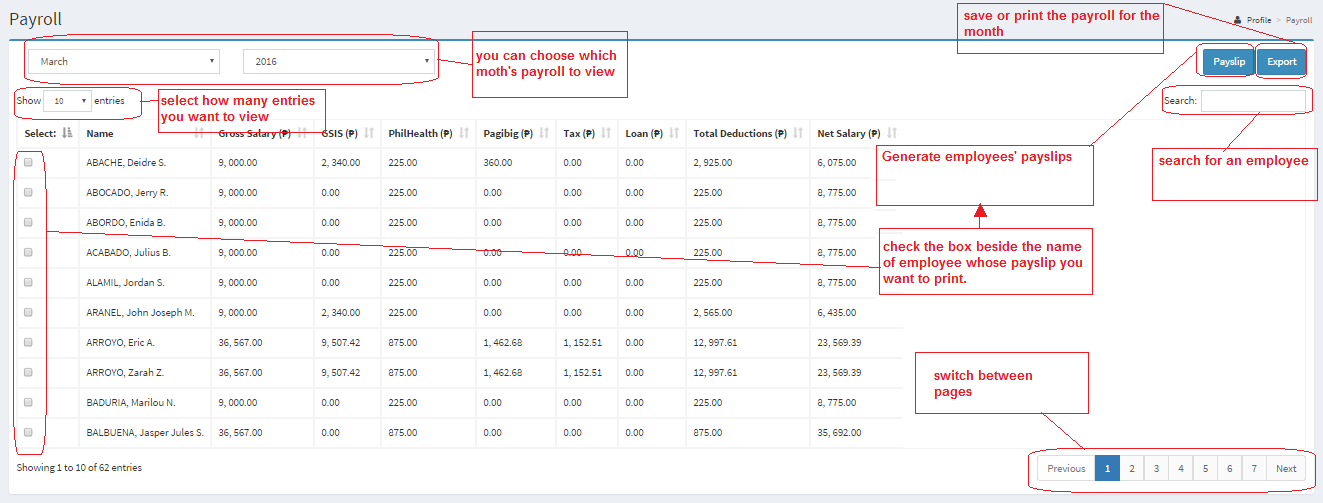
\includegraphics[width=14cm,height=7cm]{image/Payroll.png}
	\end{center}
\end{enumerate}

\newpage
\noindent
\textbf{ 2. Main Pane \\}
\begin{center}
	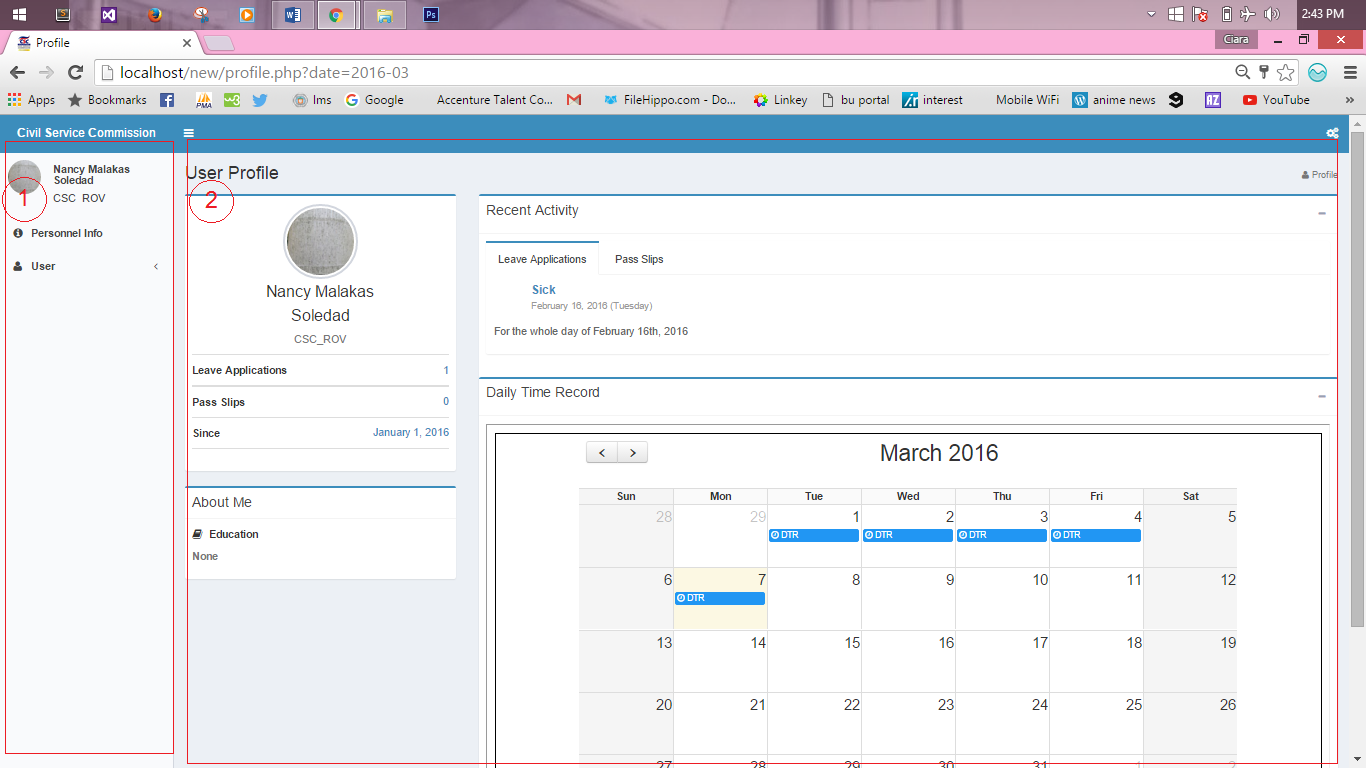
\includegraphics[width=15cm,height=7cm]{image/profile_user.png}
\end{center} 

\begin{itemize}
	\item[A.] Recent Activity
	\begin{itemize}
		\item For Users: Contains two tabs: Leave Applications, which shows a list of your filed Leave application; Pass Slips, shows a list of pass slips you filed.
		\item For Attendance Monitoring Admins and Super Admin: Contains two tabs: Leave Applications, which shows a list of all filed Leave applications for approval; Pass Slips, shows a list of pass slips filed for your approval.
	\end{itemize}
	\item Edit Personnel Data Sheet - \\ Enter all your Data, to save the data click the “Submit” button.\\
	\begin{center}
		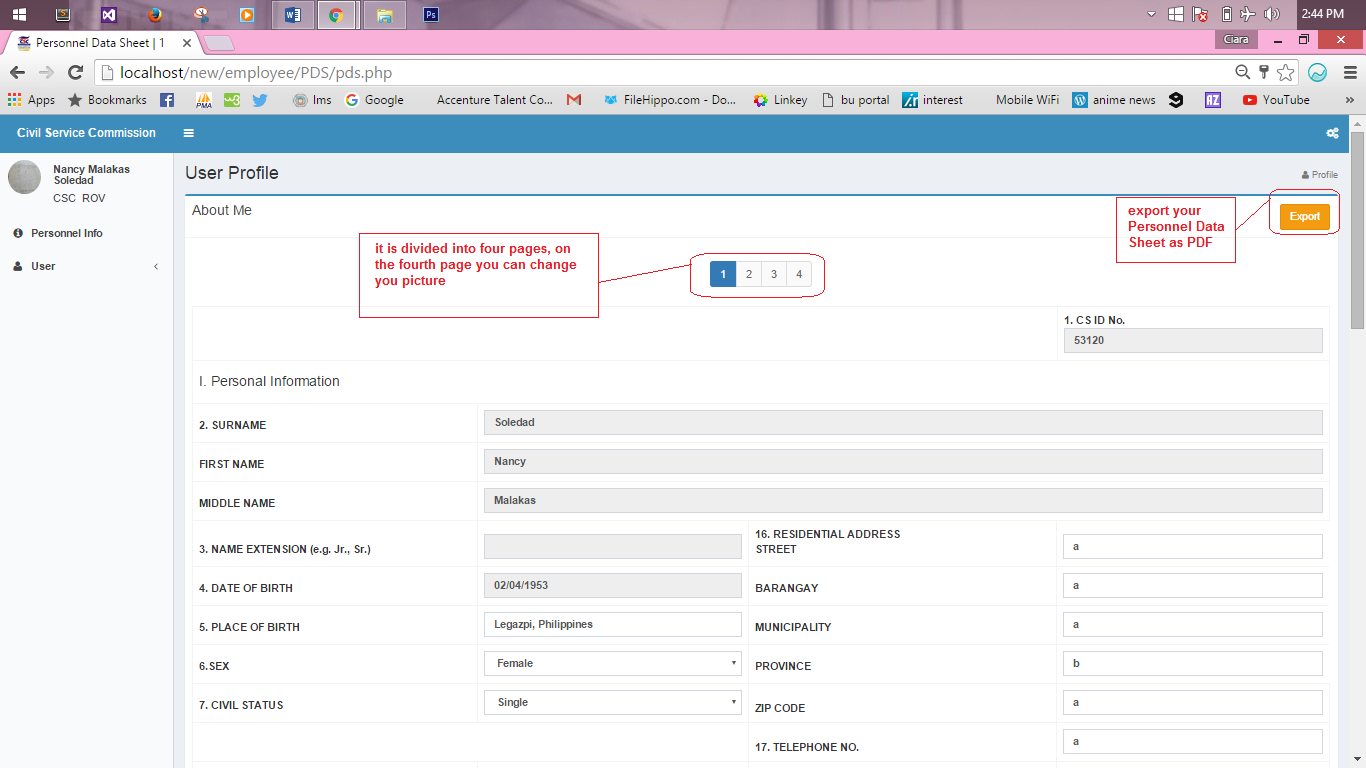
\includegraphics[width=14cm,height=8cm]{image/editPDS.png}
	\end{center} 
	\item Calendar -
	\begin{center}
		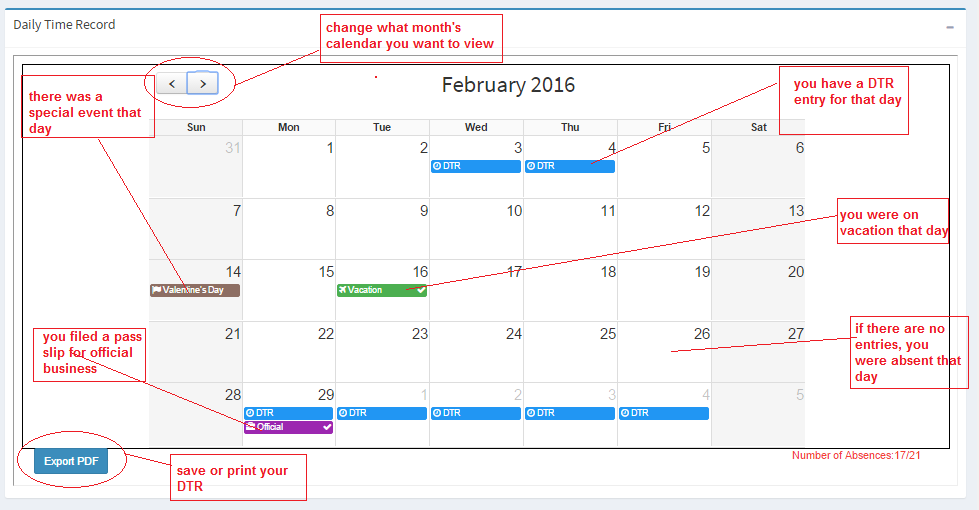
\includegraphics[width=14cm,height=7cm]{image/calendar.png}
	\end{center}
	\begin{itemize}
		\item Check Leave Credits - \\
		To check you leave credits, just click any date on the calendar.\\
		\begin{center}
			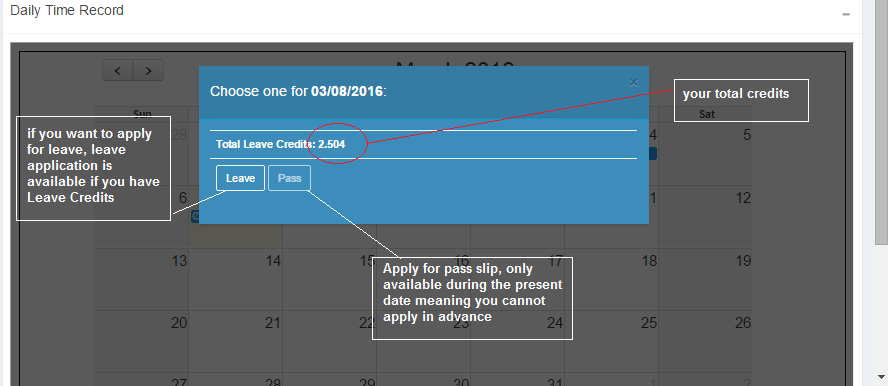
\includegraphics[width=13cm,height=8cm]{image/checkLC.png}
		\end{center} 
		\item Apply for Leave - \\
		To apply for Leave, click any date on the calendar and click the “Leave” button. A window will appear where you can enter all your leave details, click the “Submit” button for your application to filed. \\
		\begin{center}
			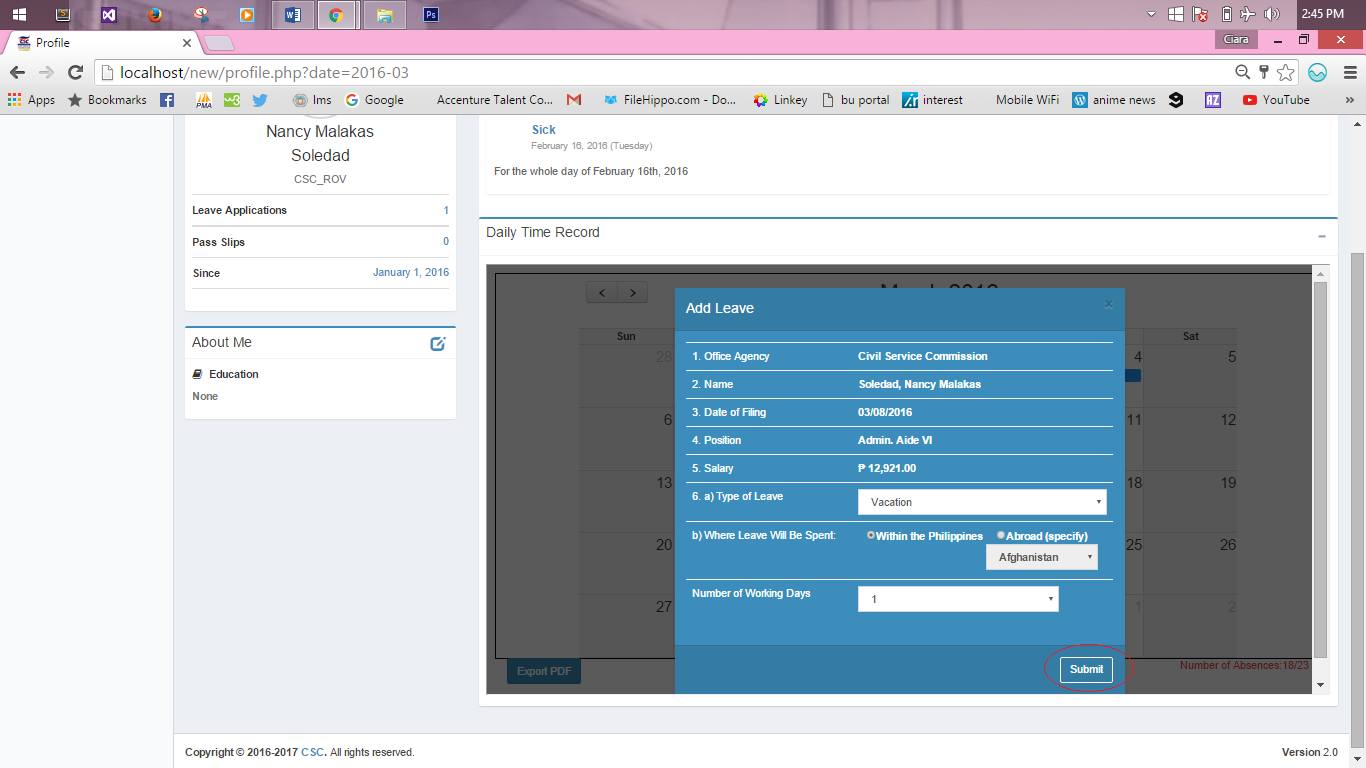
\includegraphics[width=13cm,height=8cm]{image/Leave.png}
		\end{center}
		\item Apply for Pass Slip - \\
		To apply for Pass Slips, click any date on the calendar and click the “Pass” button. A window will appear where you can enter all your pass slip details, click the “Submit” button for your application to filed. \\
		\begin{center}
			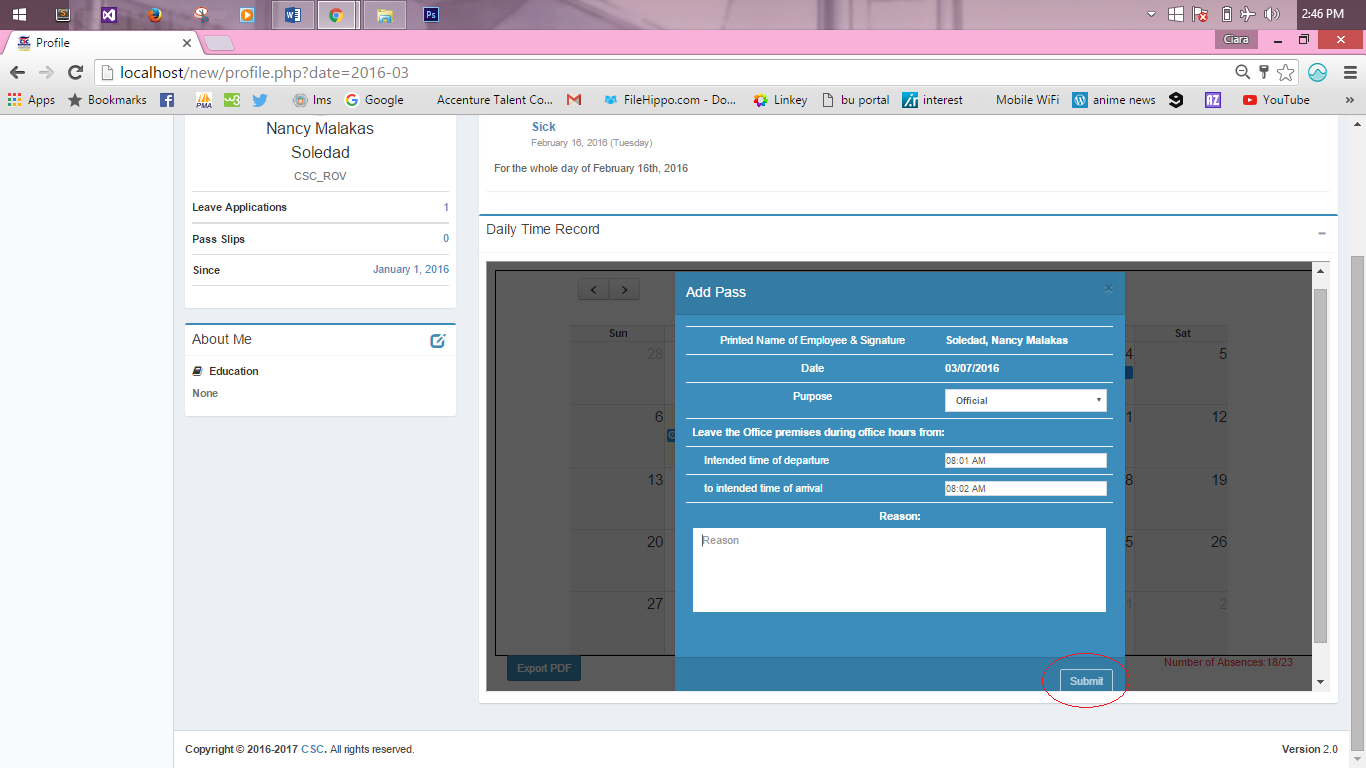
\includegraphics[width=13cm,height=8cm]{image/pass.png}
		\end{center}
		\item View Daily Time Record 
		\begin{center}
			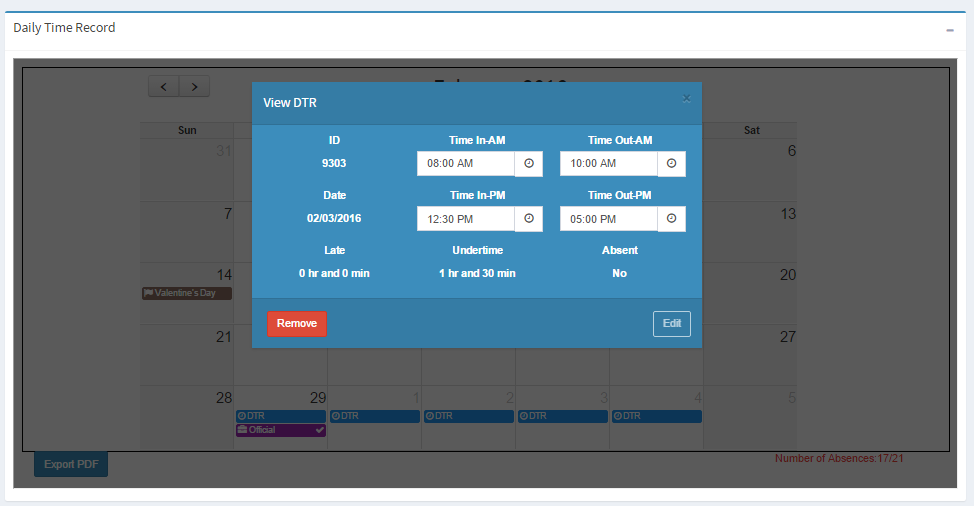
\includegraphics[width=13cm,height=8cm]{image/viewDTR.png}
		\end{center}
	\end{itemize}
\end{itemize}
